\documentclass[letterpaper,11pt]{article}

\usepackage{amsmath}
\usepackage{amssymb}
\usepackage[hmargin=1.25in,vmargin=1in]{geometry}
\usepackage{booktabs}
\usepackage{graphicx}
\usepackage{hyperref}
\usepackage{lmodern}
\usepackage{microtype}
\usepackage{pdflscape}
\usepackage{subcaption}

\title{Coursework 6: STAT 570}
\author{Philip Pham}
\date{\today}

\begin{document}
\maketitle
\begin{enumerate}
\item In this question, you will implement the algorithm you described in
  Question 4 of Exercises 5. The algorithm derived in 4(b) will now be
  implemented for the prostate cancer data. These data are available in the R
  package \texttt{lasso2} and are named \texttt{Prostate}. Take $Y$ as $\log$
  prostate specific antigen and $x$ as log cancer volume. Implement the blocked
  Gibbs sampling algorithm using the prior given in the first equation of the
  aforementioned question, with $m_0 = m_1 =0$, $v_{00} = v_{11} = 2$,
  $v_{01} = 0$, and $a=b=0$. Run two chains, one with starting values
  corresponding to the unbiased estimates of the parameters and one starting
  from a point randomly generated from the prior
  $\pi\left(\beta_0, \beta_1\right)$. Report:
  \begin{enumerate}
  \item Histogram representations of the univariate marginal distributions
    $p\left(\beta_0 \mid y\right)$, $p\left(\beta_1 \mid y\right)$ and
    $p\left(\sigma \mid y\right)$, and scatterplots of the bivariate marginal
    distributions $p\left(\beta_0, \beta_1 \mid y\right)$,
    $p\left(\beta_0,\sigma \mid y\right)$, and
    $p\left(\beta_1,\sigma \mid y\right)$.

    \begin{figure}
      \centering
      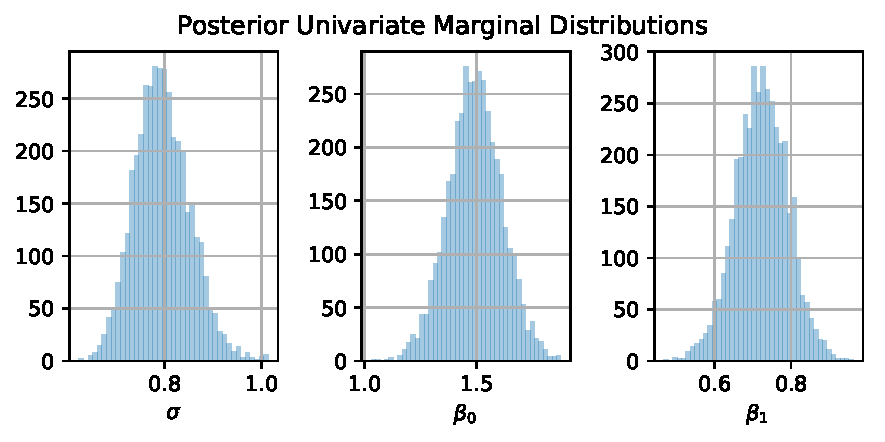
\includegraphics{p1_univariate_marginals.pdf}
      \caption{Emprical univariate distributions from Gibbs sampling.}
      \label{fig:p1_univariate}
    \end{figure}

    \begin{figure}      
      \centering
      \caption{Emprical joint distribution for
        $\left(\beta_0,\beta_1\right) \mid y$ from Gibbs sampling.}
      \label{fig:p1_beta0_beta1}
      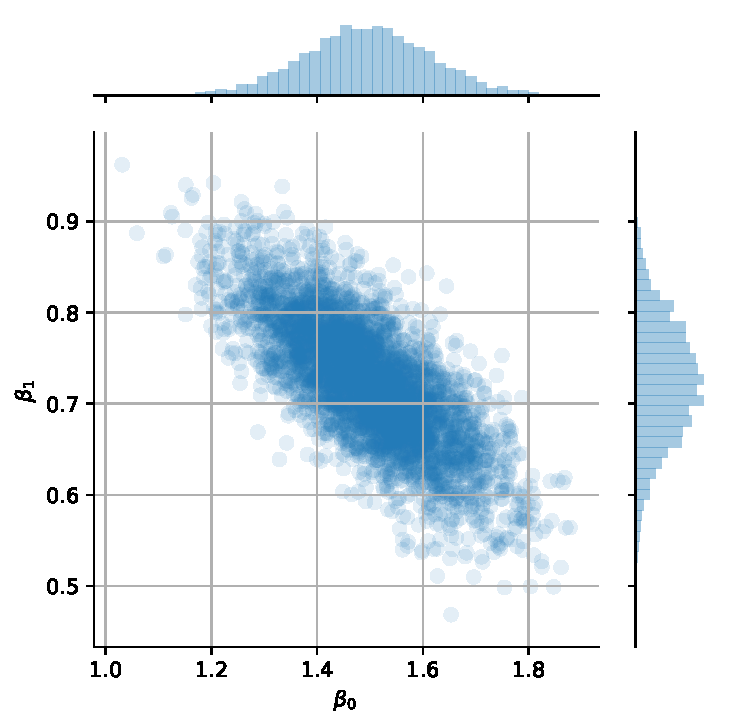
\includegraphics{p1_beta0_beta1.pdf}
    \end{figure}

    \begin{figure}      
      \centering
      \caption{Emprical joint distribution for
        $\left(\beta_0, \sigma\right) \mid y$ from Gibbs sampling.}
      \label{fig:p1_beta0_sigma}
      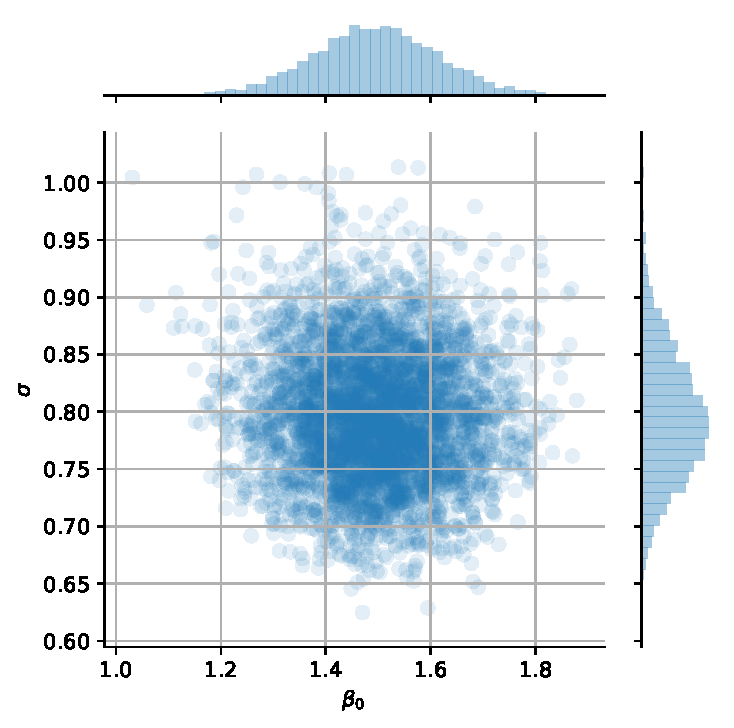
\includegraphics{p1_beta0_sigma.pdf}
    \end{figure}

    \begin{figure}      
      \centering
      \caption{Emprical joint distribution for
        $\left(\beta_1, \sigma\right) \mid y$ from Gibbs sampling.}
      \label{fig:p1_beta1_sigma}
      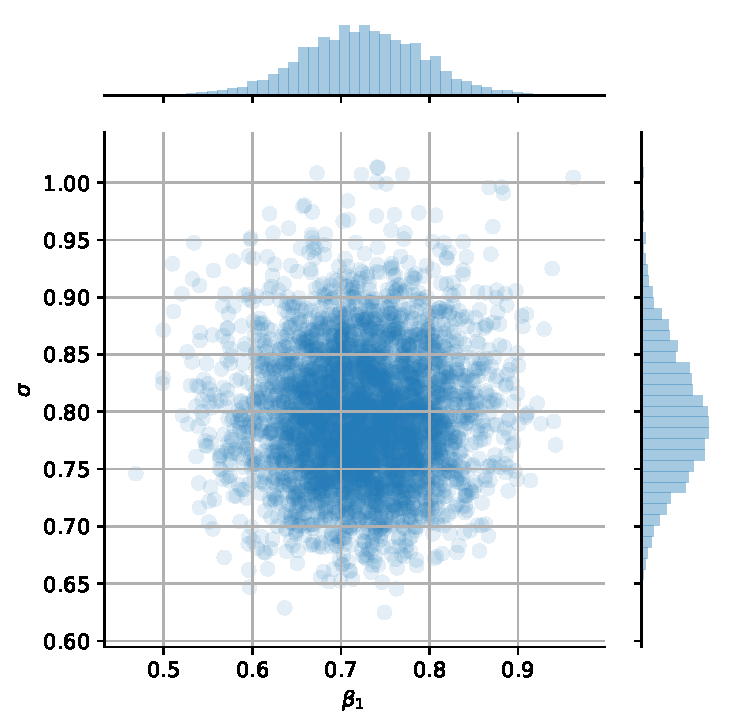
\includegraphics{p1_beta1_sigma.pdf}
    \end{figure}

    
    \begin{description}
    \item[Solution:] The empirical univariate distributions from Gibbs sampling
      can be found in Figure \ref{fig:p1_univariate}. The joint distributions
      are found in Figures \ref{fig:p1_beta0_beta1}, \ref{fig:p1_beta0_sigma},
      and \ref{fig:p1_beta1_sigma}.

      From the univariate distributions in Figure \ref{fig:p1_univariate}, we
      get samples close to the MLE estimates (see Table 5.3 of Wakefield's
      \emph{Bayesian and Frequentist Regression Methods}). The dataset is rather
      large, so this is not surprising. The distributions for $\beta_j$ are
      symmetrical. The distribution for $\sigma$ seems to skew slightly to the
      right.

      From the bivariate distributions in Figures \ref{fig:p1_beta0_sigma} and
      \ref{fig:p1_beta1_sigma}, we see that there is not much correlation
      between the $\beta_j$ and $\sigma$, which is expected since $\sigma$ is an
      ancillary statistic in the frequentist setting.

      From Figure \ref{fig:p1_beta0_beta1}, we see a negative correlation
      between $\beta_0$ and $\beta_1$, which is also expected since if we
      discount the effect of $x$ on $y$, the estimate for $\beta_0$ must
      compensate.
      
      Code for the Gibbs sampler and plots can be found at
      \href{http://nbviewer.jupyter.org/github/ppham27/stat570/blob/master/hw6/prostate.ipynb}{\texttt{prostate.ipynb}}.
    \end{description}
  \item The posterior means, standard deviations and 10\%, 50\%, 90\% quantiles
    of $\beta_0$, $\beta_1$, and $\sigma$.
    
    \begin{table}
      \small
      \centering
      \begin{tabular}{lrrrrr}
\toprule
{} &  Posterior mean &  Standard deviation &  10\% quantile &  50\% quantile &  90\% quantile \\
\midrule
$\sigma$  &        0.796154 &            0.056701 &      0.726527 &      0.793442 &      0.871269 \\
$\beta_0$ &        1.495039 &            0.120843 &      1.341545 &      1.494805 &      1.652094 \\
$\beta_1$ &        0.723290 &            0.068159 &      0.638009 &      0.724150 &      0.808873 \\
\bottomrule
\end{tabular}

      \caption{Summary statistics calculated from samples drawn with Gibbs
        sampling.}
      \label{tab:p1_summary}
    \end{table}
    
    \begin{description}
    \item[Solution:] The summary statistics for the empirical posterior
      distributions can be found in Table \ref{tab:p1_summary}. Samples from
      both chains were used for a total 4,096 samples.

      Both the posterior mean and standard deviation agree closely with the MLE
      estimates in Table 5.3 of Wakefield's \emph{Bayesian and Frequentist
        Regression Methods}. From the quantiles, we get an empirical estimate of
      the 80\% credible interval, which appear to be symmetrical with respect to
      the median.
    \end{description}
  \item $\mathbb{P}\left(\beta_1 > 0.5 \mid y\right)$
    \begin{description}
    \item[Solution:] One way to interpret the significance of $x$'s effect on
      $y$ is to look at the distribution of $\beta_1$. The emprical estimate for
      $\mathbb{P}\left(\beta_1 > 0.5 \mid y\right)$ is $\boxed{0.9990}$, so the
      effect is likely significant, both statistically and in size.

      This was calculated simply by taking the proportion of samples of
      $\beta_1$ that exceeded $0.5$. See
      \href{http://nbviewer.jupyter.org/github/ppham27/stat570/blob/master/hw6/prostate.ipynb}{\texttt{prostate.ipynb}}
      for the calculation.
    \end{description}
  \item Justify your choice of \emph{burn-in} period. For example, you may
    present the trace plots $\beta_0^{(t)}$, $\beta_1^{(t)}$,
    $\left(\log\sigma^{2}\right)^{(t)}$ versus $t$.

    \begin{figure}
      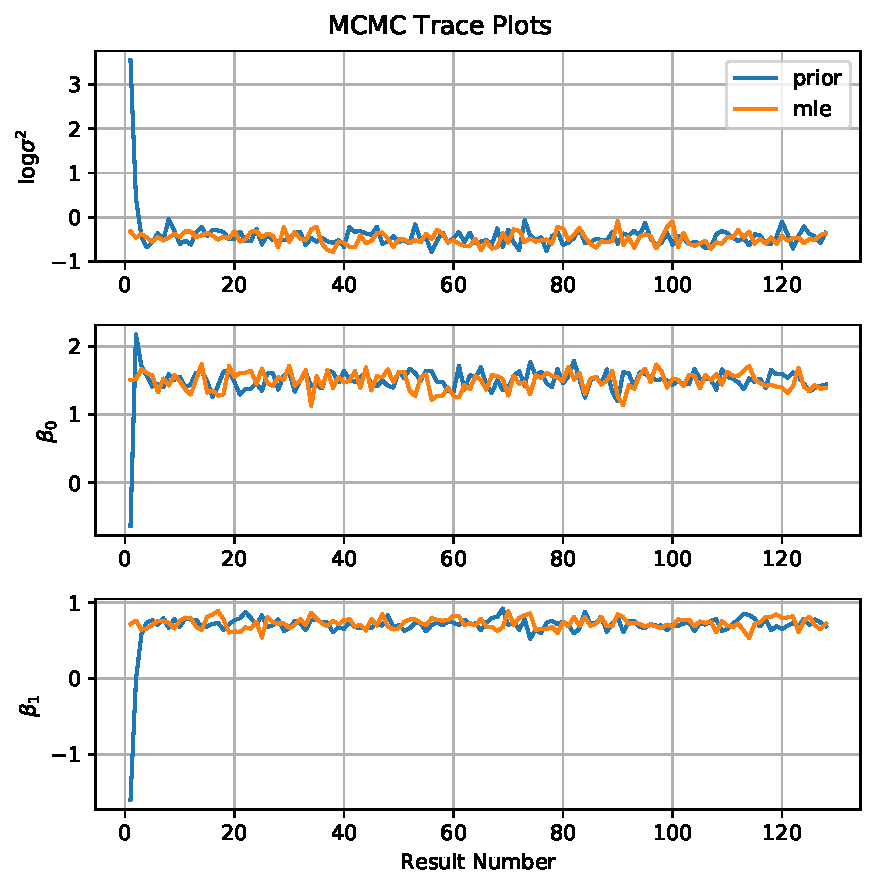
\includegraphics{p1_trace.pdf}
      \caption{The trace plots show the sampled posterior parameters at each
        step in the MCMC chain.}
      \label{fig:p1_trace}
    \end{figure}
    
    \begin{description}
    \item[Solution:] The trace plots for $\log\sigma^2$, $\beta_0$, and
      $\beta_1$ are shown in Figure \ref{fig:p1_trace}. The first 128 results
      are plotted. The MLE chain immediately is stationary. The prior chain
      quickly becomes stationary in about 10 steps.

      I specified a burn-in period of 128 steps for good measure. Then, I took
      2,048 samples from each chain with no thinning.
    \end{description}
  \end{enumerate}

  \pagebreak
\item Consider the data in Table \ref{tab:p2_data} contain data on a typical
  reliability experiment and give the failure stresses (in GPa) of four samples
  of carbon fibers of lengths 1, 10, 20 and 50mm.

  \begin{table}
    \tiny
    \centering
    \begin{tabular}{rrrrrrrrrrrrrr}
\toprule
 Length (mm) &      0 &      1 &      2 &      3 &      4 &      5 &      6 &      7 &      8 &      9 &     10 &     11 &     12 \\
\midrule
           1 &  2.247 &  2.640 &  2.842 &  2.908 &  3.099 &  3.126 &  3.245 &  3.328 &  3.355 &  3.383 &  3.572 &  3.581 &  3.681 \\
          10 &  1.901 &  2.132 &  2.203 &  2.228 &  2.257 &  2.350 &  2.361 &  2.396 &  2.397 &  2.445 &  2.454 &  2.454 &  2.474 \\
          20 &  1.312 &  1.314 &  1.479 &  1.552 &  1.700 &  1.803 &  1.861 &  1.865 &  1.944 &  1.958 &  1.966 &  1.997 &  2.006 \\
          50 &  1.339 &  1.434 &  1.549 &  1.574 &  1.589 &  1.613 &  1.746 &  1.753 &  1.764 &  1.807 &  1.812 &  1.840 &  1.852 \\
\bottomrule
\end{tabular}

    \caption{Failure stress data for four groups of fibers.}
    \label{tab:p2_data}
  \end{table}

  \begin{enumerate}
  \item Consider a Bayesian analysis with a Weibull likelihood and independent
    lognormal priors,
    $\eta \sim \operatorname{LogNormal}\left(\mu_\eta, \sigma_\eta\right)$,
    $\alpha \sim \operatorname{LogNormal}\left(\mu_\alpha,
      \sigma_\alpha\right)$. Choose $\mu_\eta$, $\sigma_\eta$ so that the prior
    probability that $\eta$ lies between 0.5 and 30 is 0.9, and $\mu_\alpha$,
    $\sigma_\alpha$ so that the prior probability that α lies between 1 and 4 is
    0.9.

    \begin{description}
    \item[Solution:]
      $\log\eta \sim \mathcal{N}\left(\mu_\eta, \sigma_\eta\right)$ by
      definition of the lognormal distribution. Since $\log$ is a monotonic
      transformation,
      \begin{align}
        0.9 = \mathbb{P}\left(1/2 \leq \eta \leq 30\right)
        &= \mathbb{P}\left(\log\frac{1}{2} \leq \log\eta \leq \log 30\right) \nonumber\\
        &=
          \mathbb{P}\left(
          \Phi^{-1}\left(0.05\right) \leq
          \frac{\log\eta - \mu_\eta}{\sigma_\eta} \leq
          \Phi^{-1}\left(0.95\right)
          \right),
          \label{eqn:p2_prior_prob}
      \end{align}
      where $\Phi$ is the cumulative distribution function of a standard normal.

      Equation \ref{eqn:p2_prior_prob} implies that
      \begin{align*}
        \frac{\log\left(1/2\right) - \mu_\eta}{\sigma_\eta}
        &= \Phi^{-1}\left(0.05\right) \\
        \frac{\log 30 - \mu_\eta}{\sigma_\eta}
        &= \Phi^{-1}\left(0.95\right).
      \end{align*}

      Solving, we have that
      \begin{align*}
        \sigma_\eta
        &=
          \frac{\log 30 - \log\frac{1}{2}}{\Phi^{-1}\left(0.95\right) - \Phi^{-1}\left(0.05\right)} 
          \approx 1.2446 \\
        \mu_\eta
        &= \log 30 - \sigma_\eta \Phi^{-1}\left(0.95\right) =
          \log \frac{1}{2} - \sigma_\eta\Phi^{-1}\left(0.05\right)
          \approx 1.3540
      \end{align*}

      Repeating the calculating for $\alpha$, we have
      $\mu_\alpha \approx 0.6931$ and $\sigma_\alpha \approx 0.4214$.

      Calculations can be found in
      \href{http://nbviewer.jupyter.org/github/ppham27/stat570/blob/master/hw6/failure\_stresses.ipynb}{\texttt{failure\_stresses.ipynb}}.
    \end{description}
  \item Run MCMC for summarizing the posterior
    $p\left(\eta, \alpha \mid y\right)$, and implement this algorithm for each
    of the groups in Table \ref{tab:p2_data}. Report the posterior medians and
    90\% credible intervals for $\eta$ and $\alpha$ and give histograms
    representations of the posterior margins for $\eta$ and $\alpha$, and a
    scatterplot representation of $p\left(\eta, \alpha \mid y\right)$.

    \begin{figure}
      \centering
      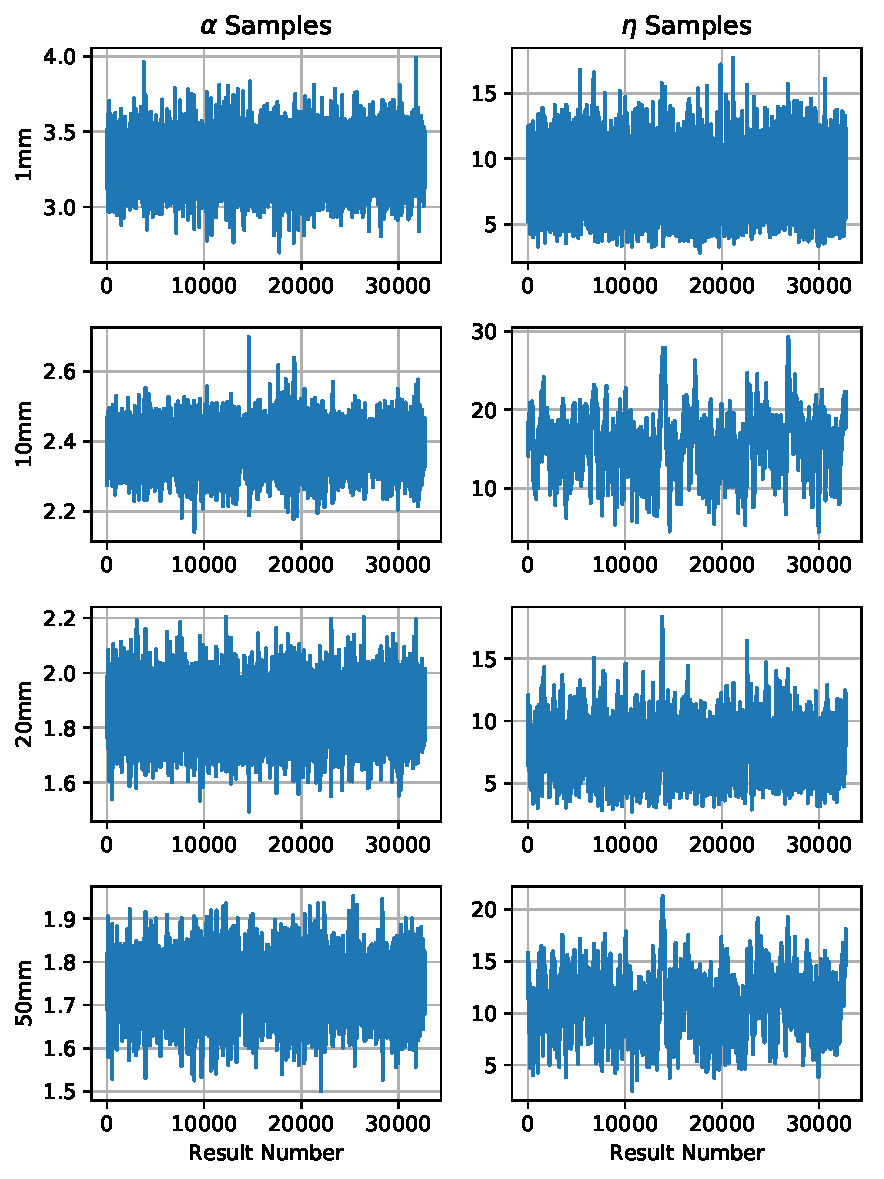
\includegraphics{p2_trace.pdf}
      \caption{Trace plots for the MCMC samples of the Weibull parameters.}
      \label{fig:p2_trace}
    \end{figure}

    \begin{figure}
      \centering
      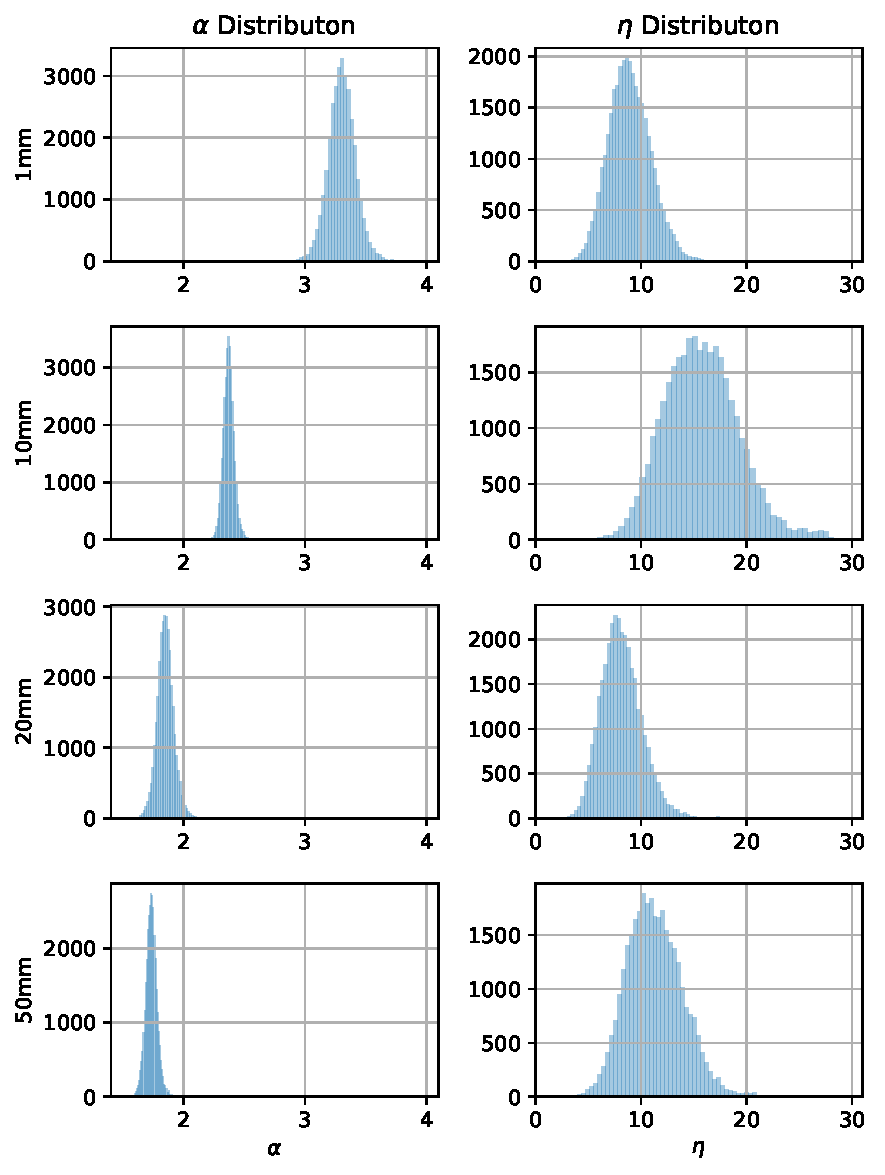
\includegraphics{p2_univariate.pdf}
      \caption{Samples from MCMC were used to approximate the posterior
        distribution of the parameters.}
      \label{fig:p2_univariate}
    \end{figure}

    \begin{figure}
      \centering
      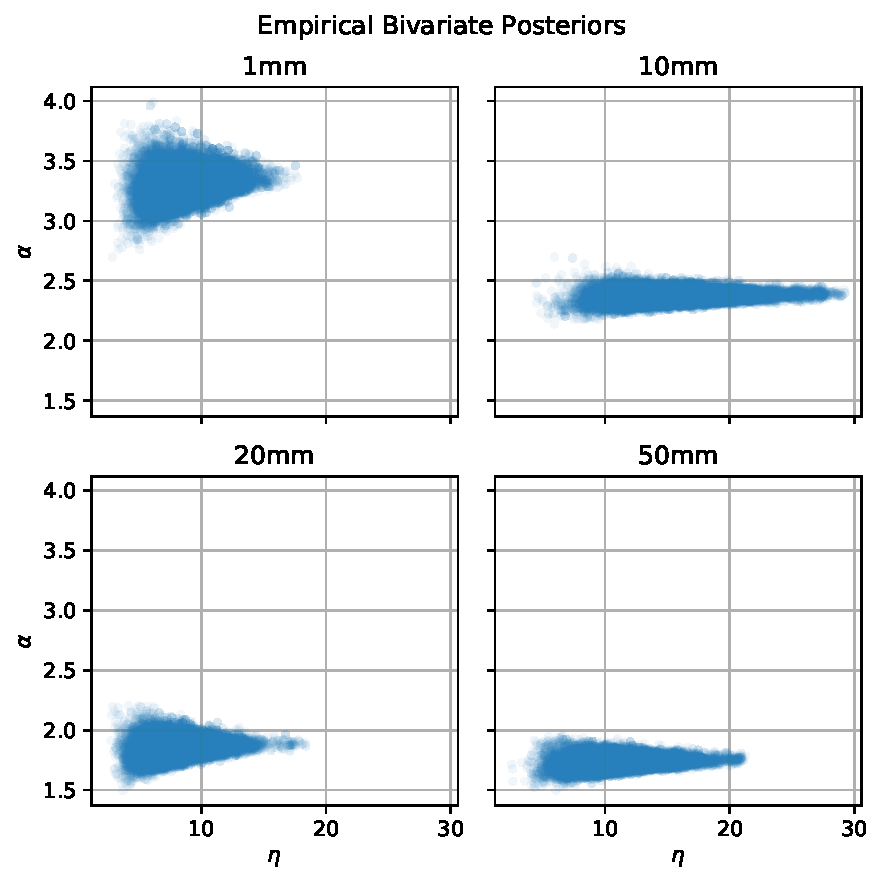
\includegraphics{p2_bivariate.pdf}
      \caption{Correlation between the parameters can be estimated with
        empirical joint distribution.}
      \label{fig:p2_bivariate}
    \end{figure}

    \begin{table}
      \scriptsize
      \centering
      \begin{tabular}{llrrrrr}
\toprule
   &        &       Mean &  Standard deviation &     Median &  5\% quantile &  95\% quantile \\
Length (mm) & Parameter &            &                     &            &              &               \\
\midrule
1  & $\alpha$ &   3.304722 &            0.113267 &   3.303521 &     3.122608 &      3.490909 \\
   & $\eta$ &   8.945404 &            1.989280 &   8.837034 &     5.846150 &     12.363148 \\
10 & $\alpha$ &   2.369973 &            0.045122 &   2.369507 &     2.298008 &      2.443862 \\
   & $\eta$ &  15.779253 &            3.575655 &  15.611898 &    10.309790 &     21.820534 \\
20 & $\alpha$ &   1.849104 &            0.069687 &   1.847223 &     1.738584 &      1.965827 \\
   & $\eta$ &   8.176279 &            1.934859 &   8.019274 &     5.281827 &     11.535180 \\
50 & $\alpha$ &   1.732334 &            0.047075 &   1.731810 &     1.656464 &      1.810707 \\
   & $\eta$ &  11.302895 &            2.636021 &  11.133819 &     7.279310 &     15.768627 \\
\bottomrule
\end{tabular}

      \caption{Posterior estimates of summary statistics calculated from the
        MCMC samples.}
      \label{tab:p2_summary}
    \end{table}
    
    \begin{description}
    \item[Solution:] For each length, 32,768 MCMC samples were generated with
      Hamiltonian Monte Carlo. Some thinning was used: 2 steps were skipped
      between each sample.

      The trace plots can be seen in Figure \ref{fig:p2_trace}. A significant
      number of burn-in steps (65,536) were needed before the distribution
      became stationary.

      The empirical univariate distributions can be found in Figure
      \ref{fig:p2_univariate}. The lognormal assumption seems appropriate.

      The empirical joint distributions can be found in Figure
      \ref{fig:p2_bivariate}. There is a triangle shape: as the shape parameter
      $\eta$ increases there is less variance in the estimate of $\alpha$.

      Posterior summary statistics can be found in Table
      \ref{tab:p2_summary}. The 90\% credible interval can be taken from the
      last two columns. These numbers are similar to the MLEs calculated in
      Homework 3, but pulled towards the prior means and and standard
      deviation. Since the number of samples is small the prior has a
      significant effect.

      Code to run the MCMC chain and recreate the plots can be found in
      \href{http://nbviewer.jupyter.org/github/ppham27/stat570/blob/master/hw6/failure\_stresses.ipynb}{\texttt{failure\_stresses.ipynb}}.
    \end{description}
  \end{enumerate}
  
  \pagebreak
\item The data in Table \ref{tab:p3_data}, taken from Wakefield et al. (1994),
  were collected following the administration of a single 30mg dose of the drug
  Cadralazine to a cardiac failure patient. The response $y_i$ represents the
  drug concentration at time $x_i$, $i = 1,\ldots,8$. The most straightforward
  model for these data is to assume
  \begin{table}
    \centering
    \begin{tabular}{rrr}
\toprule
 $i$ &  time &  drug concentration \\
\midrule
   1 &     2 &                1.63 \\
   2 &     4 &                1.01 \\
   3 &     6 &                0.73 \\
   4 &     8 &                0.55 \\
   5 &    10 &                0.41 \\
   6 &    24 &                0.01 \\
   7 &    28 &                0.06 \\
   8 &    32 &                0.02 \\
\bottomrule
\end{tabular}

    \caption{Concentrations of the drug Cadralazine (in mg/liter, $y_i$) as a
      function of time (in hours, $x_i$), for $i = 1,\ldots,8$.}
    \label{tab:p3_data}
  \end{table}

  \begin{equation}
    \log y_i = \mu\left(\beta\right) + \epsilon_i =
    \log\left[
      \frac{D}{V}\exp\left(-k_e x_i\right)
    \right]
    + \epsilon_i
    \label{eqn:p3_model}
  \end{equation}
  where
  $\epsilon_i \mid \sigma^2 \sim_\mathrm{iid}
  \mathcal{N}\left(0,\sigma^2\right)$,
  $\beta = \begin{pmatrix}V & k_e \end{pmatrix}^\intercal$ and the dose is
  $D = 30$. The parameters are the volume of distribution $V > 0$ and the
  elimination rate $k_e$.
  \begin{enumerate}
  \item For this model obtain expressions for:
    \begin{enumerate}
    \item The log-likelihood function $l\left(\beta, \sigma^2\right)$.
    \item The score function $S\left(\beta, \sigma^2\right)$.
    \item The expected information matrix $I\left(\beta, \sigma^2\right)$.
    \end{enumerate}

    \begin{description}
    \item[Solution:] We have that
      \[
        \frac{\log y_i - \log D + \log V + k_ex_i}{\sigma} = \epsilon_i \sim
        \mathcal{N}\left(0, 1\right),
      \]
      so $Y_i \sim \operatorname{LogNormal}\left(
        \log D - \log V -  k_e x_i, \sqrt{\sigma^2}\right)$      
      so the log-likelihood function is
      \begin{align}
        &l \left(\beta, \sigma^2\right)
        =\log L\left(\beta, \sigma^2\right)
          = \sum_{i=1}^n \log p\left(y_i \mid x_i, \beta, \sigma^2\right)
          \label{p3:log_likelihood} \\
        &= -\frac{n}{2}\log\left(2\pi\right)
          - \sum_{i=1}^n \log y_i
          - \frac{n}{2}\log\sigma^2
          - \frac{1}{2\sigma^2}\sum_{i=1}^n \left(\log y_i - \log D +
          \log V + k_e x_i\right)^2, \nonumber
      \end{align}
      where $n = 8$.

      Taking the gradient of Equation \ref{p3:log_likelihood}, we find the score
      function
      \begin{align}
        S\left(\beta\right)
        &= \nabla^\intercal l\left(\beta, \sigma^2\right) \nonumber\\
        &= \begin{pmatrix}
          -\frac{1}{V\sigma^2}\sum_{i=1}^n \left(y_i - \log D +
            \log V + k_e x_i\right) \\
          -\frac{1}{\sigma^2}\sum_{i=1}^n x_i\left(y_i - \log D +
            \log V + k_e x_i\right) \\
          -\frac{n}{2\sigma^2} + \frac{1}{2\left(\sigma^2\right)^2}
          \sum_{i=1}^n \left(y_i - \log D + \log V + k_e x_i\right)^2
        \end{pmatrix}.
        \label{eqn:p3_score_function}
      \end{align}

      Let $\delta_i\left(\beta\right) = y_i - \log D + \log V + k_e x_i$ and
      $RSS\left(\beta\right) = \sum_{i=1}^n
      \left[\delta_i\left(\beta\right)\right]^2.$ The expected information
      matrix can also be calculated from Equation \ref{p3:log_likelihood}
      \begin{align}
        &I_n\left(\beta, \sigma^2\right)
          = -\mathbb{E}\left[\nabla\nabla^\intercal l\left(\beta, \sigma^2\right)\right]
        \label{eqn:p3_fisher_information} \\
        &= \mathbb{E}\left[\begin{pmatrix}
          \frac{n}{V^2\sigma^2} - \frac{1}{V^2\sigma^2}\sum_{i=1}^n \delta_i\left(\beta\right) &
         \frac{1}{V\sigma^2}\sum_{i=1}^n x_i &
         -\frac{1}{V\left(\sigma^2\right)^2}\sum_{i=1}^n\delta_i\left(\beta\right) \\
          \frac{1}{V\sigma^2}\sum_{i=1}^n x_i &
          \frac{1}{\sigma^2}\sum_{i=1}^n x_i^2 &
          -\frac{1}{\left(\sigma^2\right)^2}\sum_{i=1}^n x_i\delta_i\left(\beta\right) \\
          -\frac{1}{V\left(\sigma^2\right)^2}\sum_{i=1}^n\delta_i\left(\beta\right) &
          -\frac{1}{\left(\sigma^2\right)^2}\sum_{i=1}^n x_i\delta_i\left(\beta\right) &
          -\frac{n}{2\left(\sigma^2\right)^2} +
          \frac{1}{\left(\sigma^2\right)^3}RSS\left(\beta\right)
          \nonumber
        \end{pmatrix}\right]. \\
        &= \sum_{i=1}^n\begin{pmatrix}
          \frac{1}{V^2\sigma^2} & \frac{1}{V\sigma^2}x_i & 0 \\
          \frac{1}{V\sigma^2}x_i & \frac{1}{\sigma^2}x_i^2 & 0 \\
          0 & 0 & \frac{1}{2\left(\sigma^2\right)^2}
        \end{pmatrix}. \nonumber
      \end{align}
      since $\mathbb{E}\left[RSS\left(\beta\right)\right] = n\sigma^2$ and
      $\mathbb{E}\left[S\left(\beta, \sigma\right)\right] = \mathbf{0} \implies
      \mathbb{E}\left[\delta_i\right] = 0$.
    \end{description}
  \item Obtain the MLE, and give an asymptotic 95\% confidence interval for each
    element of $\beta$.

    \begin{description}
    \item[Solution:] Let $\bar{x}$ and $\bar{y}$ be the empirical means of the
      $x_i$ and $y_i$ respectively. The MLE can be obtained from Equation
      \ref{eqn:p3_score_function}: we solve
      $S\left(\hat{\beta}, \hat{\sigma}^2\right) = \mathbf{0}$ to obtain
      \begin{align*}
        \hat{V}
        &= \exp\left(
          -\left(\bar{y} - \log D - \hat{k}_e\bar{x}\right)
          \right) \\
        \hat{k}_e
        &= -\frac{n^{-1}\sum_{i=1}^nx_iy_i - \bar{x}\bar{y}}{n^{-1}\sum_{i=1}^nx_i - \bar{x}^2}\\
        \hat{\sigma}^2
        &= \frac{1}{n}RSS\left(\hat{\beta}\right).
      \end{align*}

      The approximate covariance matrix can be obtained by inverting Equation
      \ref{eqn:p3_fisher_information}:
      \begin{align}
        \operatorname{Var}\left(\hat{\beta}, \hat{\sigma}^2\right) &\approx
        \left[I_n\left(\hat{\beta}, \hat{\sigma}^2\right)\right]^{-1} \\
        &= \begin{pmatrix}
          \frac{\hat{\sigma}^2\hat{V}^2}{n^2\hat{\operatorname{Var}}\left(X\right)}\sum_{i=1}^nx_i^2 &
          -\frac{\hat{\sigma}^2\hat{V}}{n\hat{\operatorname{Var}}\left(X\right)}\bar{x} & 0 \\
          -\frac{\hat{\sigma}^2\hat{V}}{n\hat{\operatorname{Var}}\left(X\right)}\bar{x} &
            \frac{\hat{\sigma}^2}{n\hat{\operatorname{Var}}\left(X\right)} & 0 \\
          0 & 0 & 2\frac{\left(\hat{\sigma}^2\right)^2}{n}
        \end{pmatrix}, \nonumber
      \end{align}
      where
      $\hat{\operatorname{Var}}\left(X\right) = n^{-1}\sum_{i=1}^nx_i^2 -
      \bar{x}^2$ is the empirical variance estimate of the $\left\{x_i\right\}$.
    \end{description}
    
  \item Plot the data, along with the fitted curve.
  \item Using residuals, examine the appropriateness of the assumptions of the
    above model. Does the model seem reasonable for these data?
  \item The clearance $Cl = V \times k_e$ and elimination half-life
    $x_{1/2} = \log 2/k_e$ are parameters of interest in this experiment. Find
    the MLEs of these parameters along with asymptotic 95\% confidence intervals.
  \end{enumerate}
\end{enumerate}
\end{document}
